\chapter{Hardwareumsetzung}
\label{cha:robot}
\section{Anforderungen an den NXT-Roboter}

Der Roboter hat einige hardwareseitige Anforderungen. Das System muss sich frei im Raum bewegen können, sowie eine Möglichkeit bieten mit Gegenständen zu interagieren. Diese müssen aufgehoben, transportiert und zielgerichtet abgelegt werden können. Es ist zusätzlich wichtig, dass die Gegenstände beim Ablegen sicher an ihrer Position verharren, damit sie sich nicht aus einer möglichen Zielzone heraus bewegen. Wichtiges Kriterium ist zusätzlich eine sichere Halterung für das Kameramodul, welches in Kapitel \ref{sec:Kamera} näher beschrieben ist.

\section{Entwurf des Roboters}

Da das LEGO Mindstorm NXT Kit häufig zur Realisierung kleinerer Roboterprojekte verwendet wird, hat LEGO eine Datenbank an möglichen Bauplänen bereitgestellt \cite{building_instructions}. Nach einiger Recherche und Durchsicht diverser Bauanleitungen für verschiedenste Anwendungsbereiche wurde sich für einen von LEGO bereitgestellten Aufbau den entschieden. Abbildung \ref{fig:standardRoboter} zeigt den Roboter, wie LEGO ihn bereitstellt.

\begin{figure}[h]
\centering
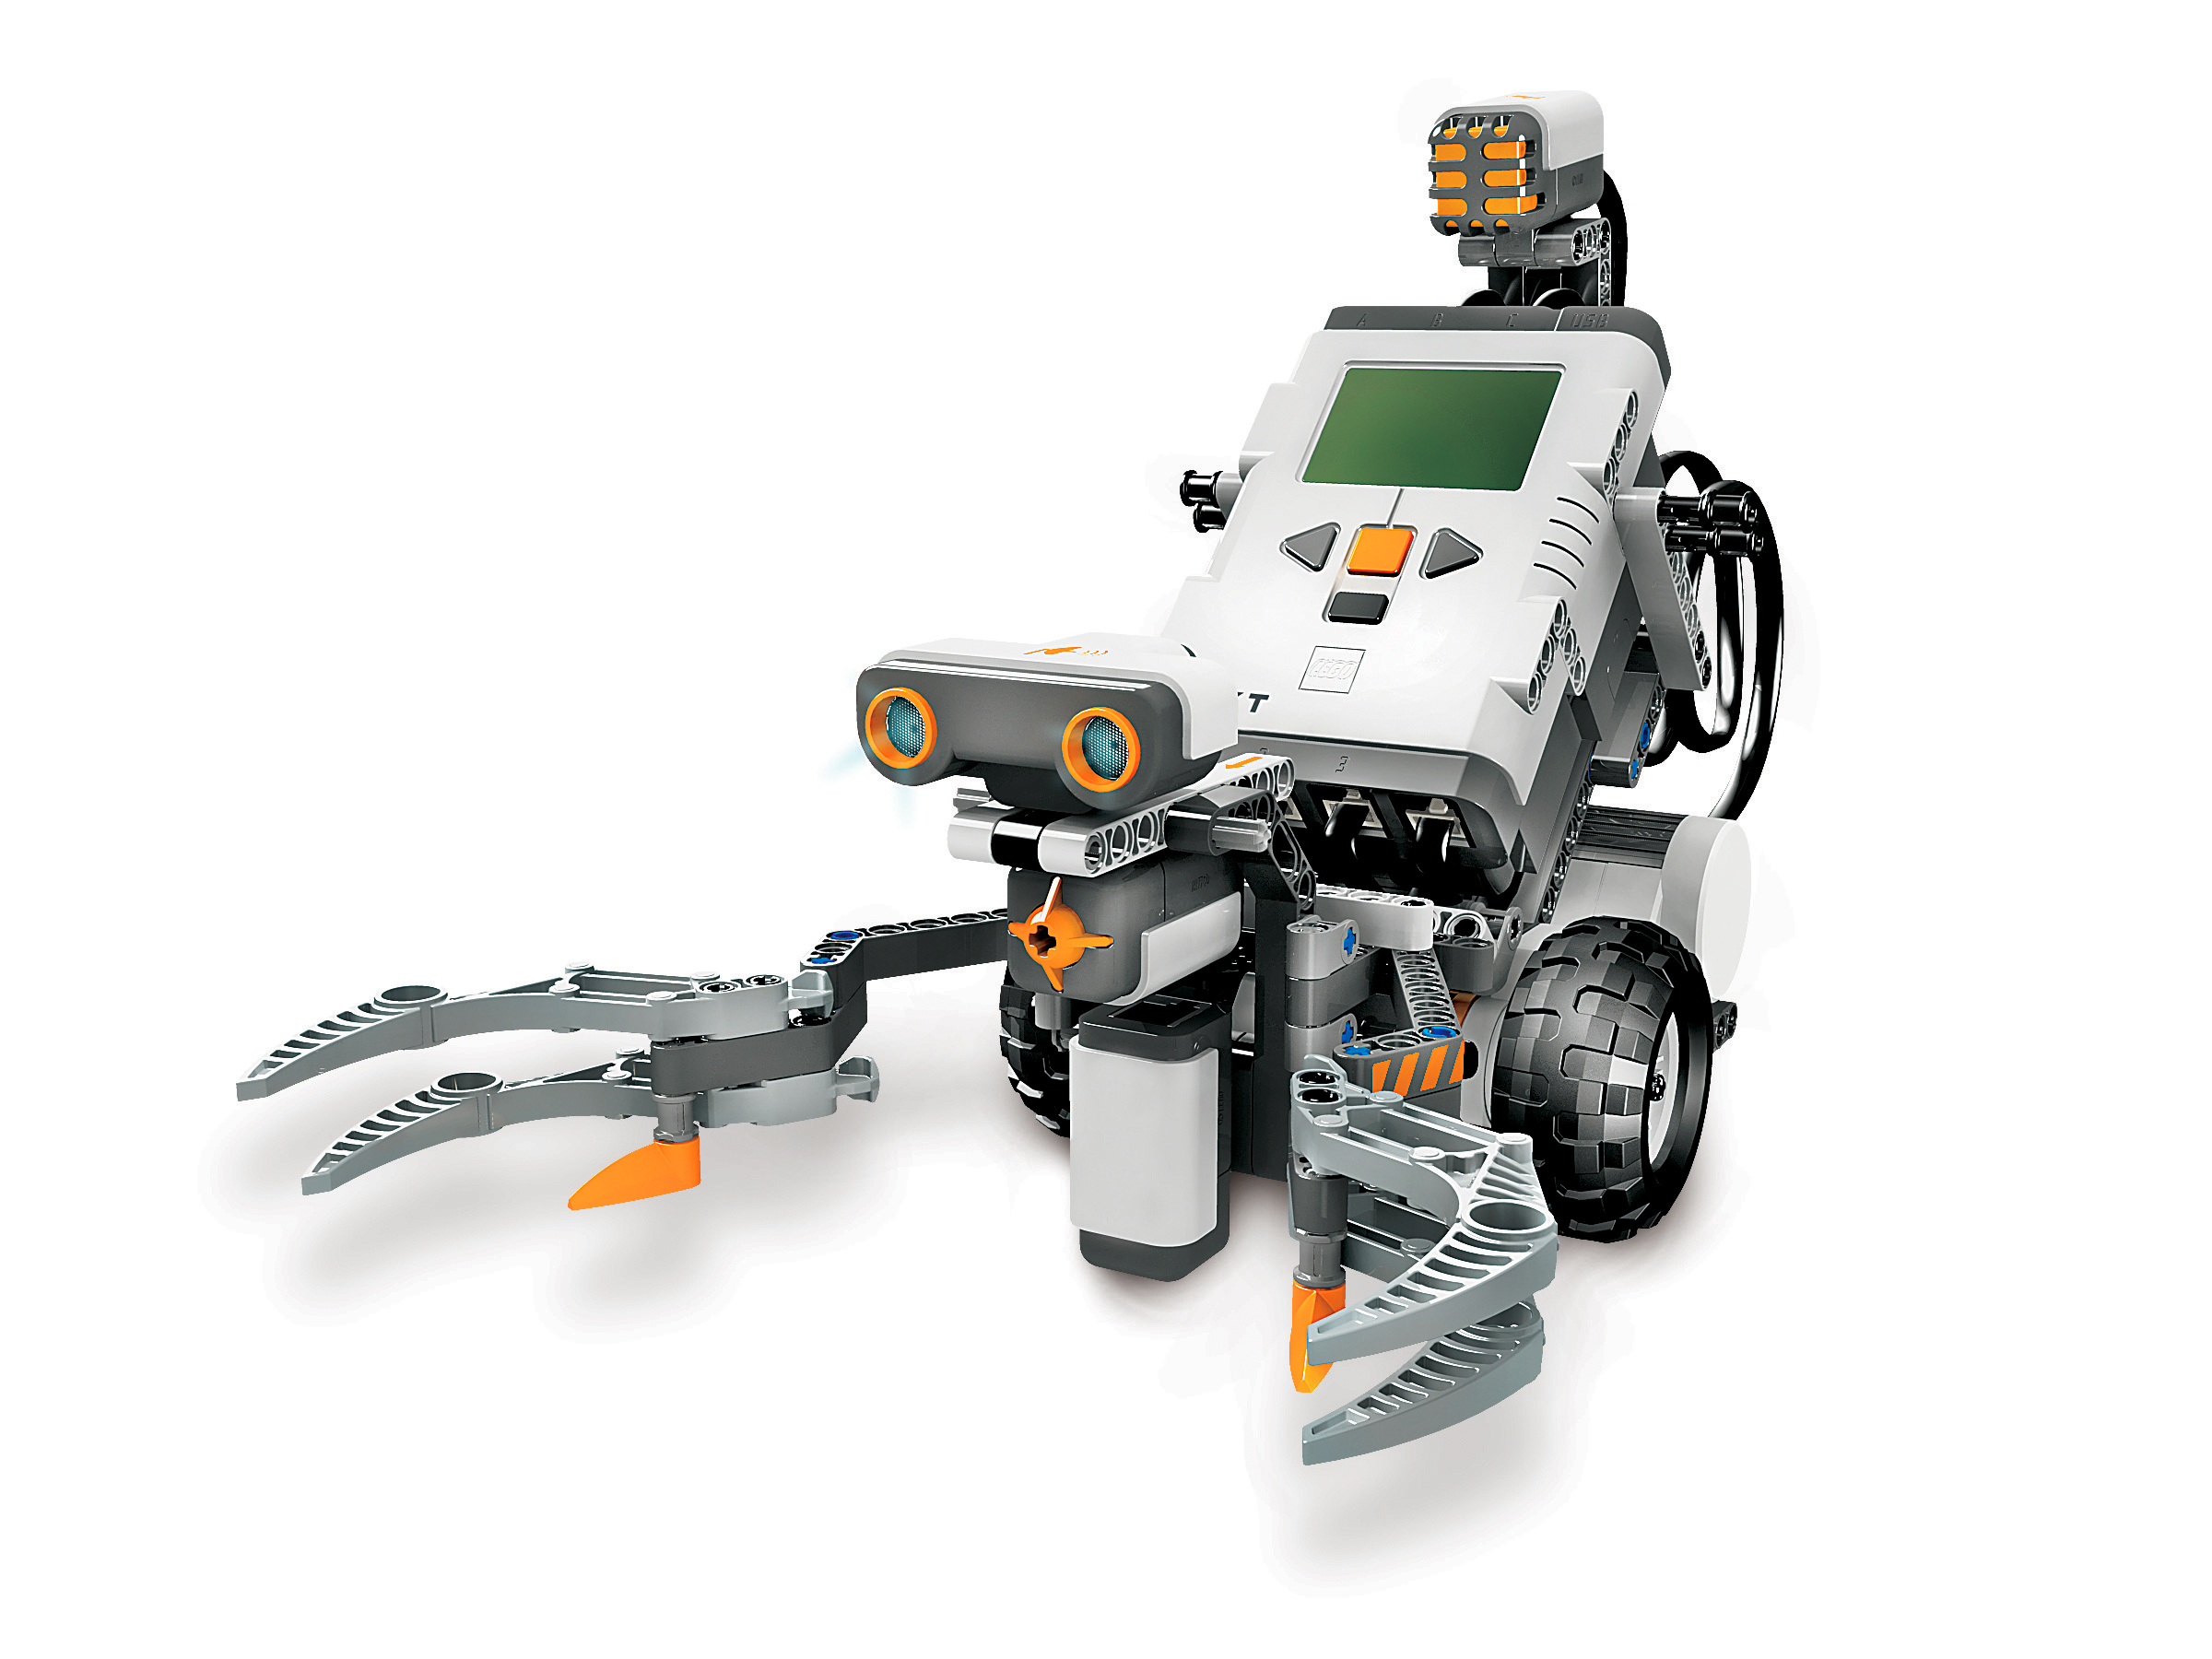
\includegraphics[width=0.8\textwidth]{Bilder/Robot/nxt_default}
\caption{Von Lego bereitgestellter Roboteraufbau}
\label{fig:standardRoboter}
\end{figure}


Da der Aufbau jedoch nicht allen Anforderungen genüge tut, wurde dieser abgeändert. Der von LEGO bereitgestellte Bauplan benutzt einen Schall- und einen Farbsensor. Diese wurden nicht benötigt und daher entfernt. An ihrer Stelle wurde stattdessen eine Halterung für das in Kapitel \ref{sec:Kamera} beschriebene Kameramodul in Form eines Smartphones eingebaut. Um dem Gewicht des Smartphones entgegenzuwirken musste der in Abschnitt \ref{subsec:Brick} beschriebene NXT-Stein etwas nach hinten verlagert werden. Abbildung \ref{fig:unserRoboter} zeigt den fertig modifizierten Roboter.

\begin{figure}[h]
\centering
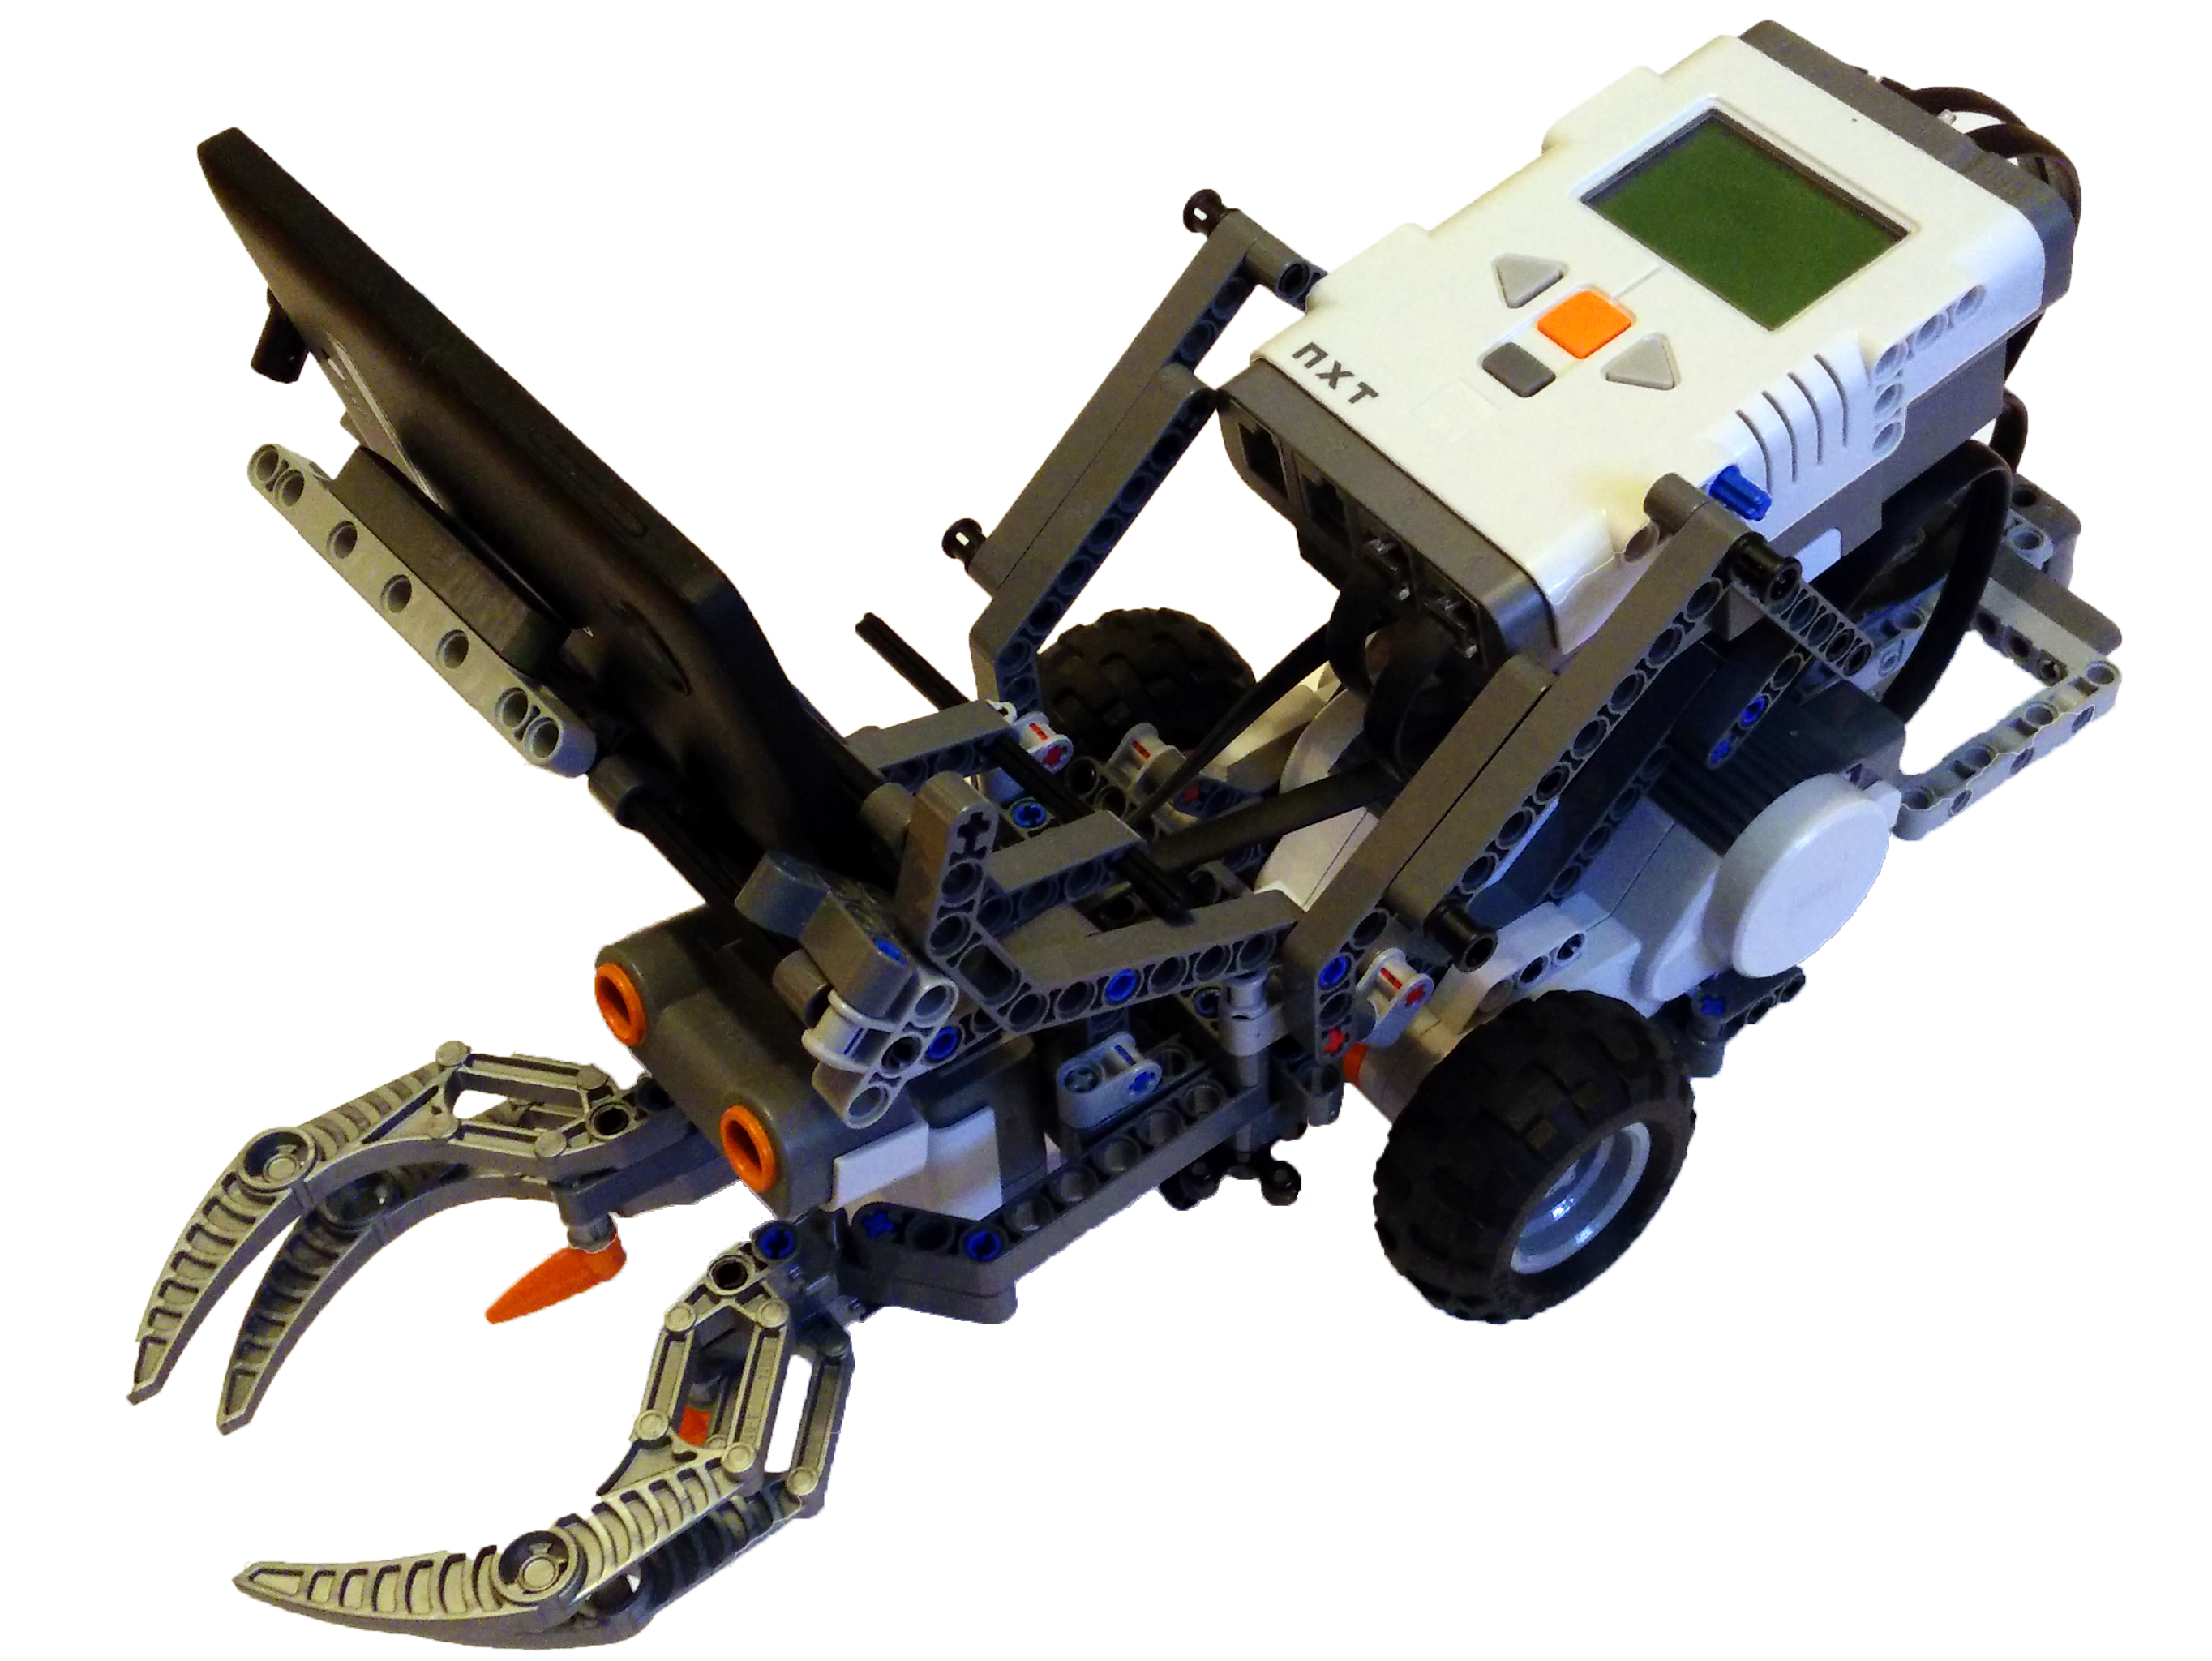
\includegraphics[width=0.8\textwidth]{Bilder/Robot/cleenr_front}
\caption{Bild des fertig modifizierten Roboters}
\label{fig:unserRoboter}
\end{figure}

\subsection{NXT-Stein}
\label{subsec:Brick}
\begin{figure}[h]
\centering
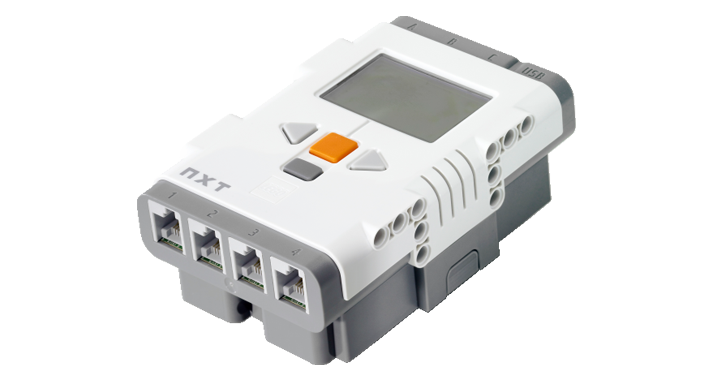
\includegraphics[width=0.5\textwidth]{Bilder/Robot/nxt_brick}
\caption{NXT-Stein}
\label{fig:nxtBrick}
\end{figure}

Der NXT-Stein bildet die Recheneinheit und damit die Hauptkomponente des Robotersystems \cite{ranganathan2008use}. Er besitzt drei Ausgänge für Motoren an der Oberseite, über die gleichzeitig die Rotationssensoren in den Servo-Motoren ausgelesen werden.

Auf der Unterseite befinden sich vier Eingänge für verschiedene Sensoren, die je nach Anwendungszweck über Flachbandkabel bestückt werden können, etwa ein Licht-, Schall-, Tastsensor oder beliebige Kombinationen daraus. Dies macht das NXT-System zu einem sehr flexiblem da einfach konfigurierbaren Robotersystem.

Über einen USB-Anschluss oben wird der NXT mit dem PC verbunden um ihn mit Programmen zu versorgen. Hierfür wird von LEGO eine graphische Entwicklungsumgebung bereitgestellt um auch Neulingen den Einstieg in die Roboter-Programmierung zu vereinfachen und ihnen die Möglichkeit zu bieten schon innerhalb weniger Minuten einen funktionierenden Prototypen zu konstruieren. Im Fall des CLEEN-R-Aufbaus wird jedoch, wie in Abschnitt \ref{sec:RoboterSteuerung} geschildert, lediglich die interne Bluetooth-Verbindung genutzt.

Auf der Vorderseite befindet sich ein $100\times 64$ Pixel auflösendes binäres LCD-Display über das Einstellungen getätigt oder Statusmeldungen ausgegeben werden können. Auch Sound-Ausgabe über einen integrierten 8-Bit-Lautsprecher ist möglich.

\subsection{Sensoren}

LEGO stellt unterschiedliche Sensoren für den Betrieb an einem NXT-Robotersystem bereit. Die wichtigsten Sensortypen sind in den nachfolgenden Abschnitten beschrieben.

\subsubsection{Tastsensor}

\begin{figure}[h]
\centering
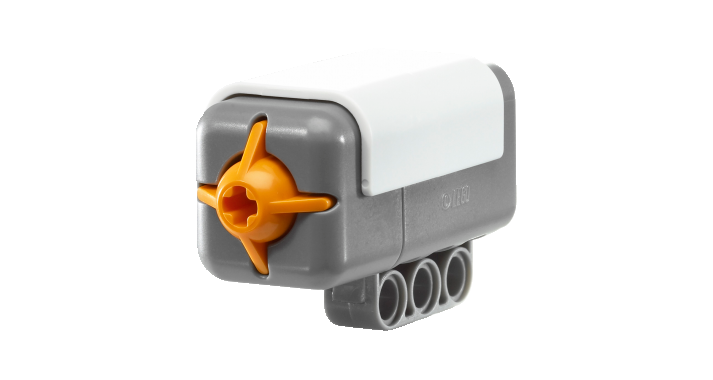
\includegraphics[width=\textwidth/3]{Bilder/Robot/button_sensor}
\caption{Tastsensor des NXT-Systems}
\label{fig:buttonSensor}
\end{figure}

Der berührungsempfindliche Tastsensor dient in der ursprünglichen Vorlage zur Detektion von Gegenständen im Bereich des Greifarms. Wird er betätigt, so kann der Greifarm geschlossen werden. Im CLEEN-R-Projekt wurde dieser jedoch durch einen Ultraschallsensor ersetzt, der nicht nur die unmittelbare Berührung bemerkt sondern auch ein herannahendes Objekt während der Fahrt detektiert. Der Ultraschallsensor ist in einem nachfolgenden Abschnitt beschrieben.

\subsubsection{Rotationssensoren}

Die Servomotoren des Roboters sind mit Rotationssensoren ausgestattet. Diese Sensoren erlauben es dem NXT-Roboter, die Geschwindigkeit der Motoren abhängig des Widerstands des Untergrunds zu regulieren. So werden unter anderem präzises Abbremsen und Fehlerminimierung bei der Positionsbestimmung ermöglicht.

\subsubsection{Farbsensor}

\begin{figure}[h]
\centering
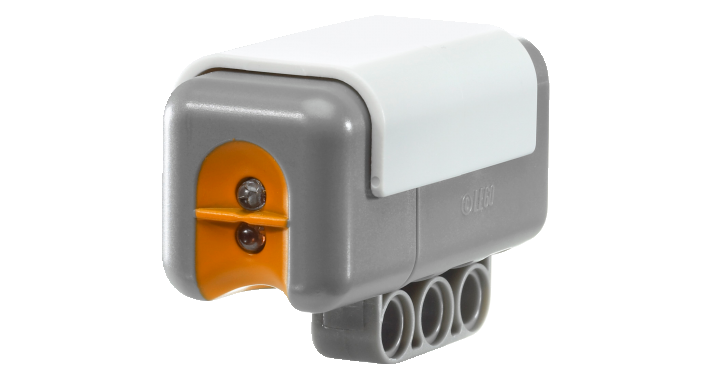
\includegraphics[width=\textwidth/3]{Bilder/Robot/color_sensor}
\caption{Farbsensor des NXT-Systems}
\label{fig:colorSensor}
\end{figure}

Dem ursprünglichen Entwurf des Roboters liegt ein RGB-Farbsensor bei. Seine Aufgabe war es die Farbe des Untergrunds festzustellen. Im CLEEN-R-Projekt wurde dieser Sensor zwar entfernt, könnte jedoch bei Erweiterung des Roboters dazu genutzt werden um die Farbe des Untergrunds aus Aufnahmen des Kameramoduls zu entfernen. Dies würde die Qualität der Objekterkennung auf farbigen Untergrund deutlich erhöhen. Zusätzlich ist es denkbar die Erkennung von Zielzonen über farbige Markierungen auf dem Untergrund zu realisieren.

\subsubsection{Ultraschallsensor}
\label{subsec:Ultraschallsensor}

\begin{figure}[h]
\centering
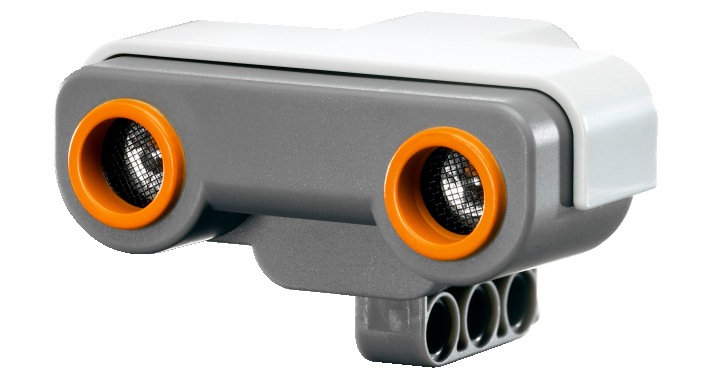
\includegraphics[width=\textwidth/3]{Bilder/Robot/distance_sensor}
\caption{Ultraschallsensor des NXT-Systems}
\label{fig:distanceSensor}
\end{figure}

Der Ultraschallsensor dient zur Messung der Distanz vom Roboter zum nächsten soliden Objekt. Der Sensor hat eine Reichweite von $255cm$ und kann mit einer Präzision von $\pm 3cm$ Entfernungen angeben. Der Sensor wird in diesem Projekt benutzt um zu detektieren, wie weit ein Objekt vom Greifarm entfernt ist. Hat es einen gewissen Abstand erreicht, so kann der Greifarm geschlossen werden um das Objekt aufzunehmen. 

In Kapitel \ref{subsec:Entfernungsschätzung} werden alternative Möglichkeiten zur Entfernungsmessung geschildert. Der Ultraschallsensor stellt sich jedoch als geeignetstes Mittel heraus und wird daher im folgenden verwendet.

\subsection{Aktoren}

Die Aktoren des Robotersystems beschränken sich beim CLEEN-R-Projekt auf Servomotoren. Im Folgenden werden die unterschiedlichen Anwendungen der Motoren beschrieben.

\subsubsection{Antriebsmotoren}

\begin{figure}[h]
\centering
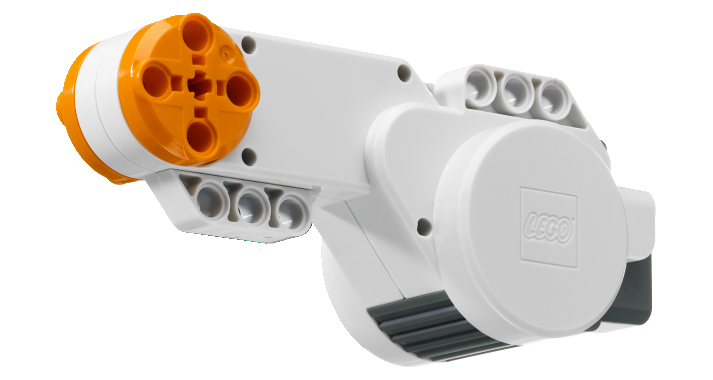
\includegraphics[width=\textwidth/3]{Bilder/Robot/motor}
\caption{Servo-Motor des NXT-Systems}
\label{fig:motor}
\end{figure}

Der NXT-Roboter verwendet zwei Servomotoren an den Seiten als Differentialantrieb. Dieser ermöglicht eine freie Fortbewegung und das Rotieren des Roboters. 

\subsubsection{Greifarm}
\label{sec:Greifarm}
Der Greifarm des Roboters wird über einen dritten Motor auf der Vorderseite bewegt. Der Motor erlaubt das freier öffnen und schließen des Greifarms und somit das mitführen von Gegenständen. 

Bei der Ansteuerung des Greifarmmotors ist zu beachten, dass dieser nicht zu schnell geschlossen werden sollte, da dies zu tragende Objekte wegstoßen könnte. Abbildung \ref{fig:Greifarm} zeigt den Greifarm in geschlossenem Zustand mit einem transportierten Objekt.

\begin{figure}[h]
\centering
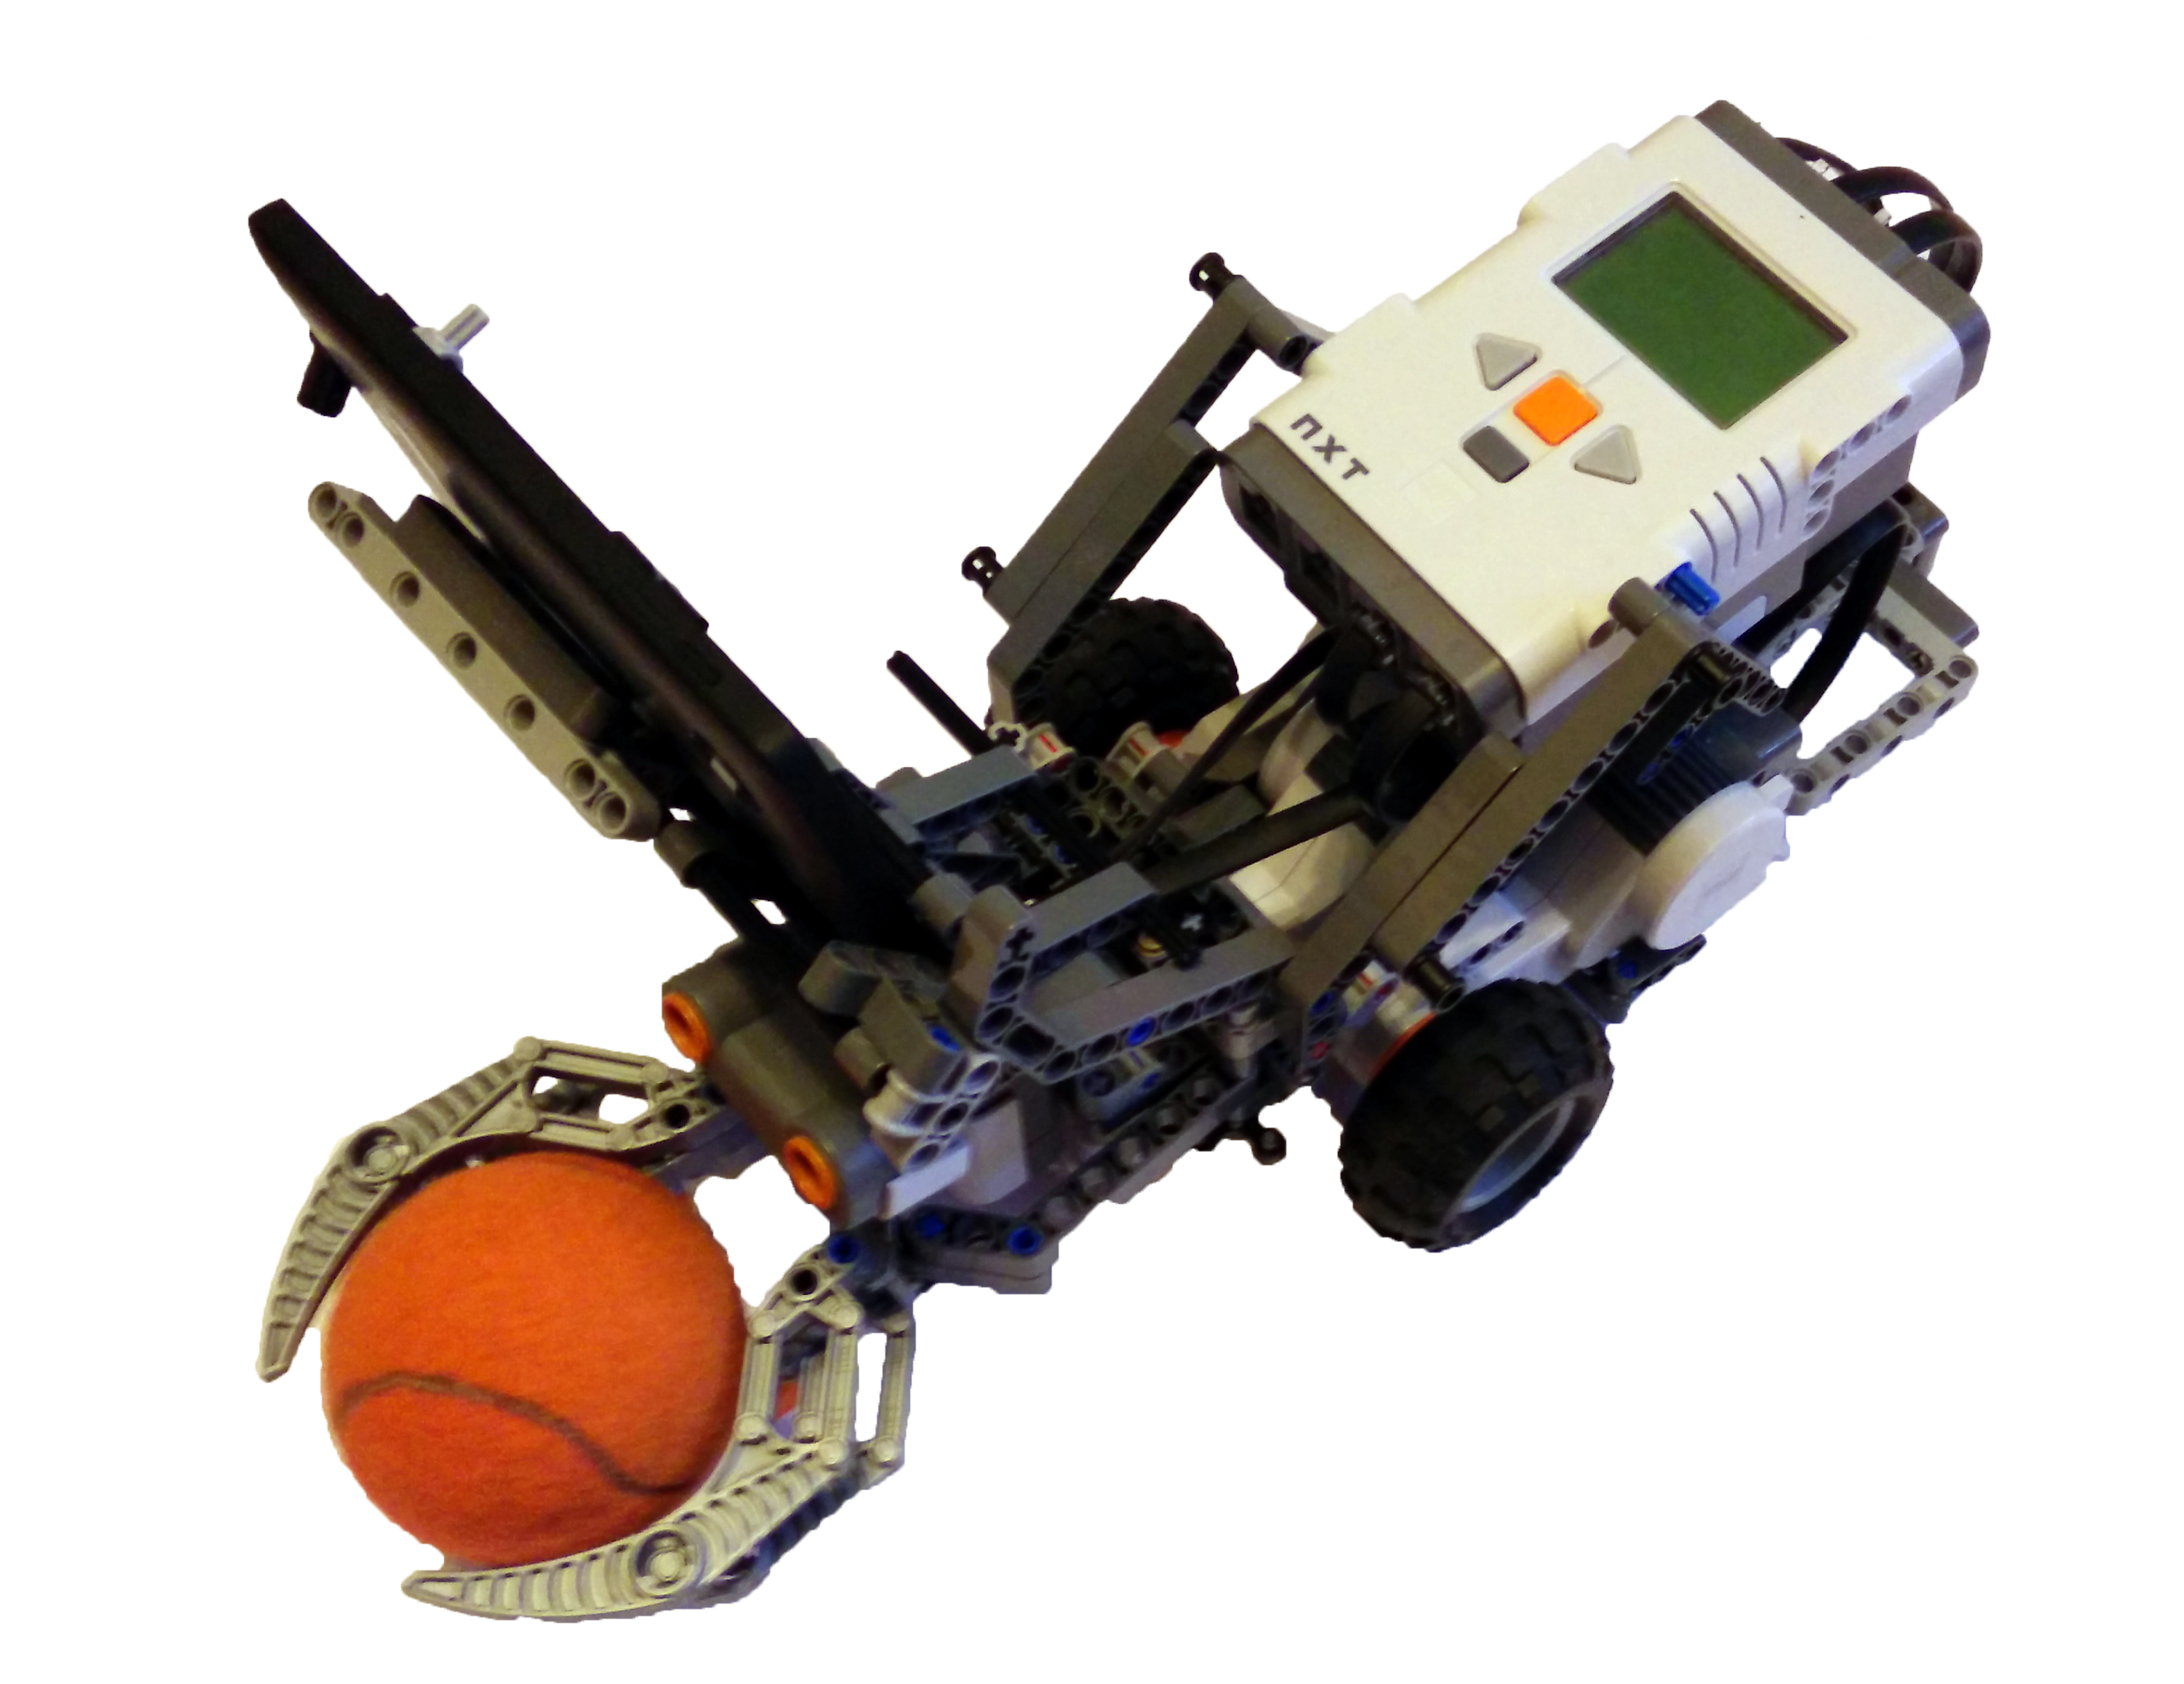
\includegraphics[width=0.8\textwidth]{Bilder/Robot/cleenr_with_object}
\caption[Greifarm des Robotersystems]{Greifarm des Robotersystems in geschlossenem Zustand mit Objekt}
\label{fig:Greifarm}
\end{figure}

\section{Steuerung des Roboters}
\label{sec:RoboterSteuerung}

Da die Kameraeinheit in Form des Smartphones und der NXT-Roboter zwei getrennte Module darstellen, ist ein nichttrivialer Kommunikationskanal notwendig. In den folgenden Abschnitten ist die intermodulare Kommunikation näher beschrieben.

\subsection{Kommunikation zwischen den Modulen}

Die Steuerung des Roboters durch das Smartphone erfolgt via Bluetooth. Der NXT-Roboter stellt hierzu als Bluetooth-Gerät das Serial Port Profile (SPP) bereit, welches das Standardinterface auf Bluetooth-Ebene darstellt und vom Großteil aller Bluetooth-Hostgeräte unterstützt wird. Es ermöglicht das simple serielle Senden und Empfangen von Bytes auf Low-Level-Ebene.

Das Kommunikationsprotokoll auf High-Level-Ebene und damit die nötigen Befehle zum Regeln der Aktoren und Auslesen der Sensoren wurde von LEGO dokumentiert und ist online erhältlich \cite{nxt_comm_protocol}.

\begin{figure}[h]
\centering
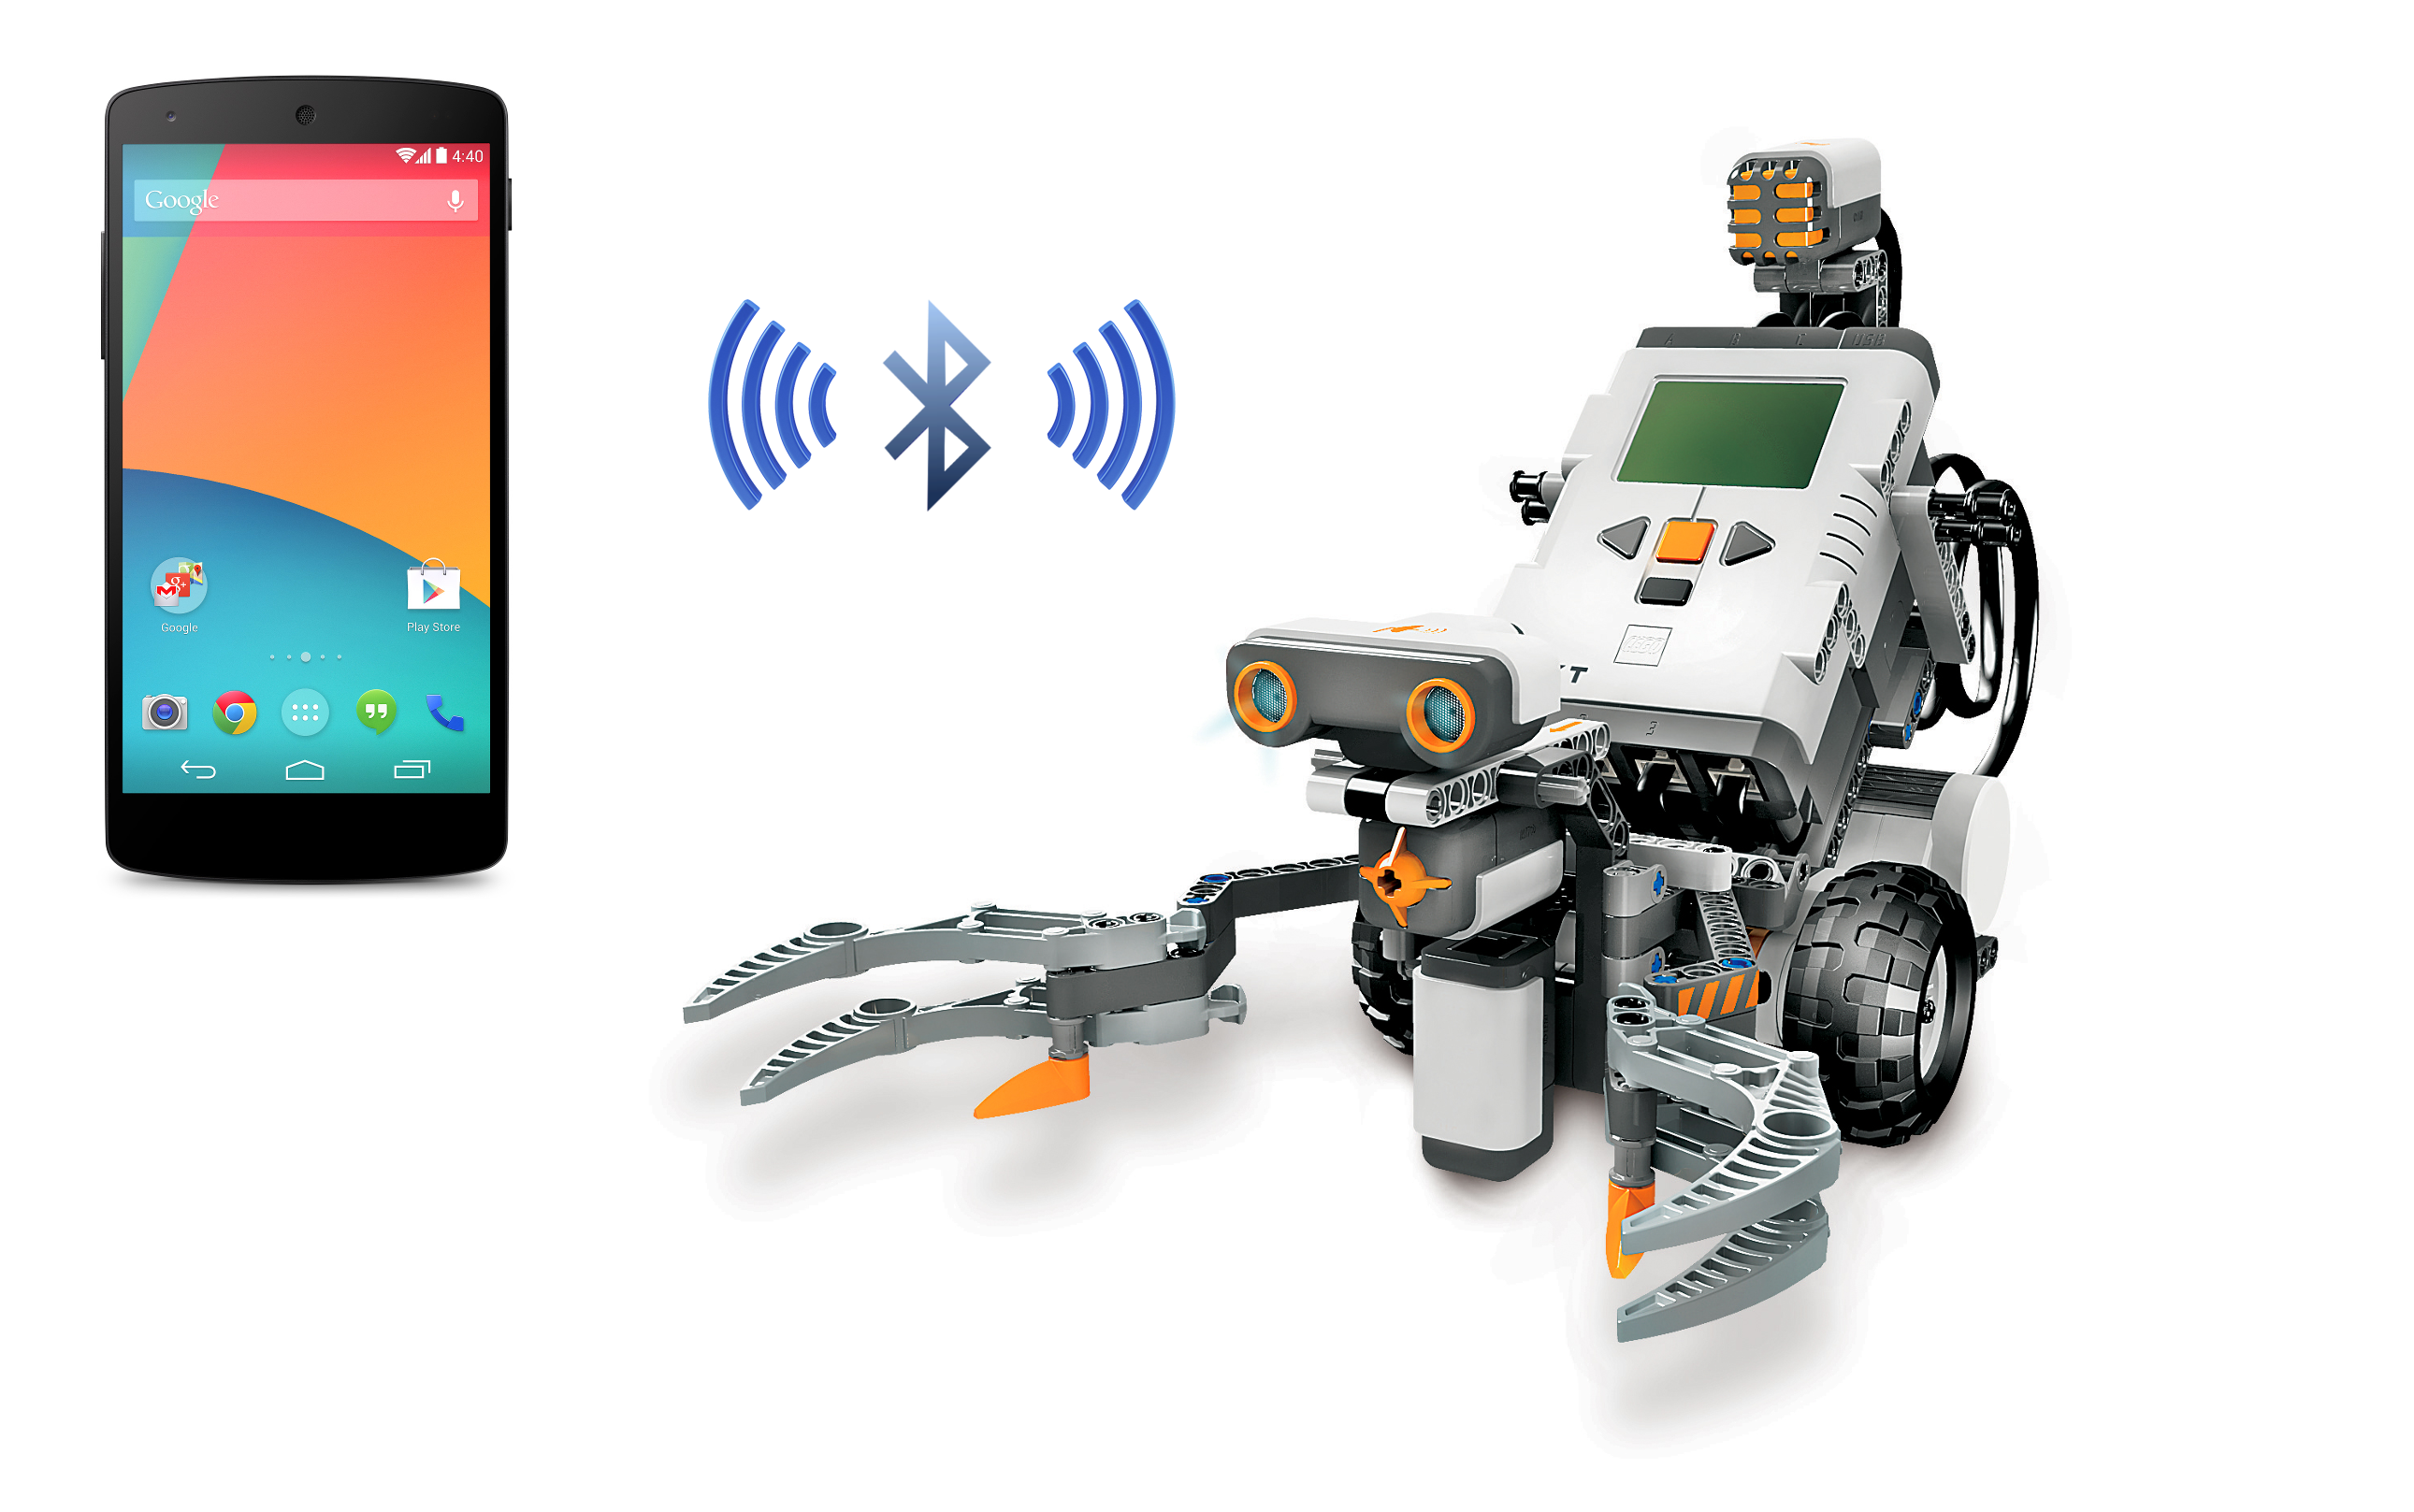
\includegraphics[width=\textwidth/2]{Bilder/Robot/bluetooth}
\caption{Bluetooth-Verbindung zwischen NXT und Nexus 5}
\label{fig:bluetooth}
\end{figure}

Um die Logik zentral zu halten wird auf dem NXT selbst kein Programm ausgeführt. Das Smartphone führt zentral alle Berechnungen durch sendet dem Roboter lediglich Befehle zur Ansteuerung der Aktoren. Sensordaten können ebenfalls durch das Smartphone über die Bluetooth-Verbindung abgerufen werden.

\subsection{Kommunikation über die Bluetooth-Schnittstelle}

Zunächst muss eine Bluetooth-Verbindung erstellt werden. Hierfür müssen beide Geräte eine aktive Bluetooth-Schnittstelle aufweisen. Der Roboter muss diese Schnittstelle zusätzlich von außen sichtbar schalten.

Bei Erstverbindung muss der gesuchte NXT ausgewählt werden. Für Folgeverbindungen ist die Bluetooth-Adresse bekannt und die App kann ohne Benutzerinteraktion eine Verbindung mit dem NXT-Roboter aufnehmen.

Ist eine Verbindung geglückt, kann damit begonnen werden seriell byteweise Befehle an den NXT zu übertragen. Eventuelle Antworten, wie beispielsweise angeforderte Sensordaten werden über die selbe Schnittstelle empfangen.

\subsection{Programmatische Umsetzung}

Auf dem Smartphone übernimmt ein gesonderter Thread die Kommunikation mit dem NXT. Die Klasse \glqq NxtTalker\grqq\ bietet Funktionen zum Versenden von Daten an den Roboter, sowie alle nötigen Daten um eine Verbindung aufzubauen und aufrecht zu erhalten.

Um die Motoren zu bewegen, muss zunächst ein Befehl an jeden Aktor geschickt werden, der eine Geschwindigkeit im Bereich von -100\% bis 100\% definiert. Hierdurch können die Motoren mit dem selben Befehl vorwärts und rückwärts fahren. Das stoppen der Motoren, und damit das Anhalten des Systems werden realisiert, indem allen Motoren eine Geschwindigkeit von null kommuniziert wird. Problematisch ist hierbei, dass die Motoren sequenziell gestartet werden. Dies hat zur Folge, dass ein Motor vor dem anderen startet und somit die Blickrichtung des Roboters beeinflusst. Um dem vorzubeugen sieht die Schnittstelle einen Befehl vor, der die Motoren synchron starten lässt. Hierdurch wird verhindert, dass der Roboter in eine undefinierte Richtung abdriftet.
